\chapter{Implementasi dan Pengujian}
\label{chap:implementasipengujian}

Pada bab ini akan dibahas mengenai hasil implementasi dan pengujian dari Open Source Snake 360.

\section{Implementasi}
Pada bagian ini akan dijelaskan mengenai lingkungan yang digunakan untuk membangun dan implementasi antarmuka dari Open Source Snake 360.

\subsection{Lingkungan Perangkat Keras}
Berikut adalah lingkungan perangkat keras yang digunakan dalam pembangunan permainan ini: 

\begin{enumerate}
	\item Perangkat : Laptop
	\item Processor : Intel Core i5-7200U 2.5GHz
	\item RAM : 4.00 GB
	\item Video Card : GeForce 930MX
	\item Monitor : 14"
	\item Storage : 1TB
\end{enumerate}

Pada pengujian digunakan 1 buah perangkat mobile berbasis android dan 1 buah perangkat desktop. Berikut adalah lingkungan perangkat keras yang digunakan dalam pengujian permainan ini:

\textbf{Perangkat 1}\\
\begin{enumerate}
	\item Perangkat : Laptop
	\item Processor : Intel Core i5-7200U 2.5GHz
	\item RAM : 4.00 GB
	\item Video Card : GeForce 930MX
	\item Monitor : 14"
	\item Storage : 1TB
\end{enumerate}

\textbf{Perangkat 2}\\
\begin{enumerate}
	\item Perangkat : SM-J730G
	\item Processor : Exynos 7870 Octa 1600MHz Cortex-A53
	\item RAM : 3.00 GB
	\item Video Card : Mali-T830
	\item Monitor : 5.5"
	\item Storage : 32 GB
\end{enumerate}

\subsection{Lingkungan Perangkat Lunak}
Berikut adalah lingkungan perangkat lunak yang digunakan dalam pembangunan permainan ini:

\begin{enumerate}
	\item Sistem Operasi Laptop : Windows 10 64-bit
	\item Bahasa Pemrograman : Javascript, HTML
	\item Sistem Operasi Smartphone : Android Nougat v7.0
\end{enumerate}

\subsection{Implementasi Antarmuka}
Pada subbab ini akan ditampilkan dan dijelaskan tampilan antarmuka dari Open Source Snake 360.

\subsubsection{Tampilan Menu Utama}
Gambar~\ref{fig:GUIUtama} merupakan tampilan antarmuka menu utama. Pada tampilan ini terdapat judul dari permainan, input untuk mengisi level dan kecepatan, dan tombol "OK". 

\begin{figure}[H]
	\centering  
	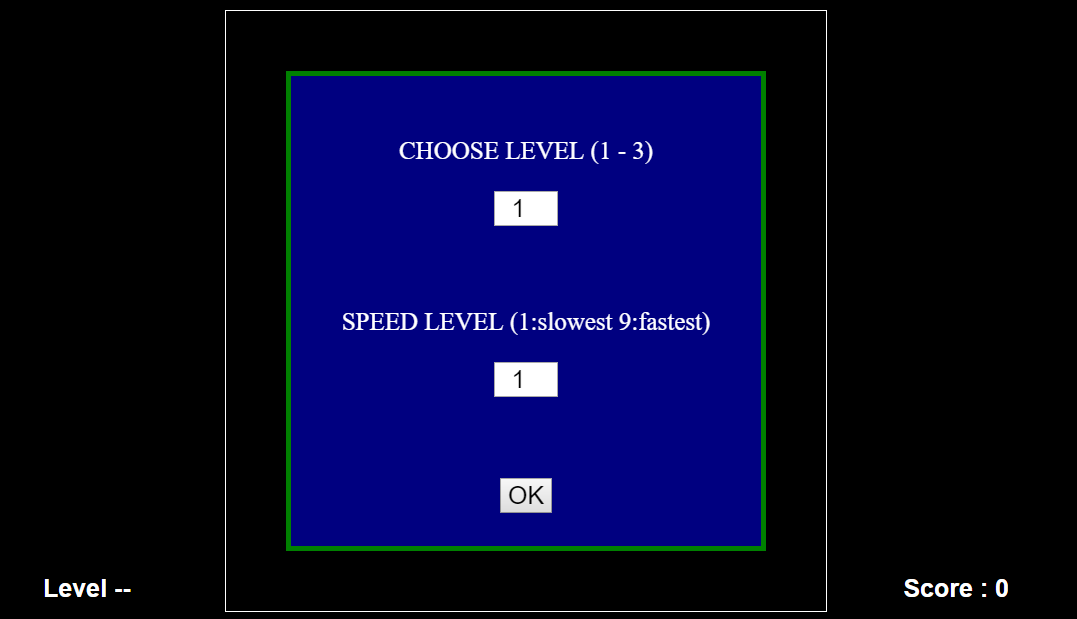
\includegraphics[scale=0.5]{GUIUtama}  
	\caption[Tampilan Menu Utama]{Tampilan Menu Utama}
	\label{fig:GUIUtama} 
\end{figure}

\subsubsection{Tampilan Bermain}
Gambar~\ref{fig:GUIBermain} merupakan tampilan antarmuka mulai bermain. Tampilan ini muncul apabila pemain memasukkan data level dan kecepatan ular dengan benar dan menekan tombol "OK". Pada tampilan ini terdapat ular yang dikontrol oleh pemain, dinding labiin, makanan ular, level labirin dan skor yang didapat pemain.

\begin{figure}[H]
	\centering  
	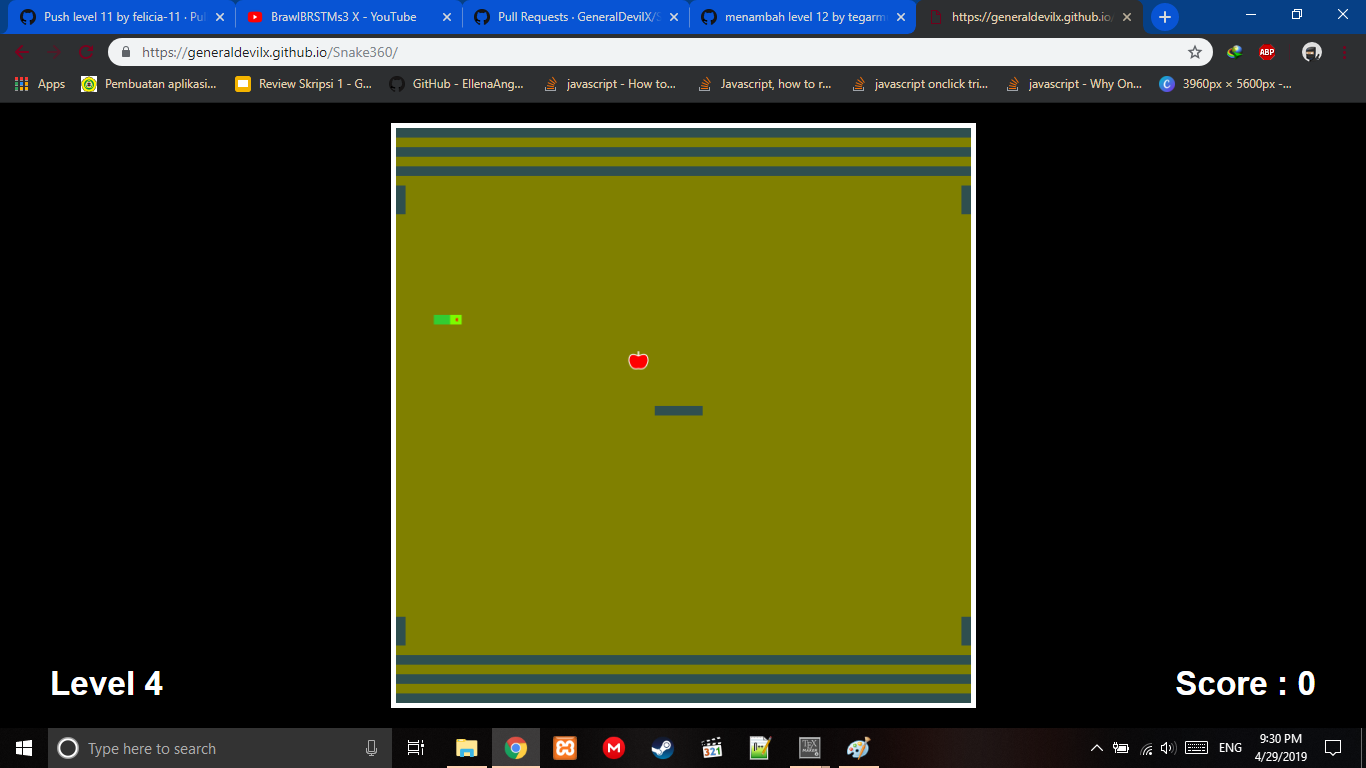
\includegraphics[scale=0.5]{GUIBermain}  
	\caption[Tampilan Bermain]{Tampilan Bermain}
	\label{fig:GUIBermain} 
\end{figure}

\section{Pengujian}
Pengujian terhadap permainan Open Source Snake 360 ini bertujuan untuk mengetahui apakah permainan yang dibangun sudah berjalan sesuai dengan rancangan. Pengujian yang dilakukan meliputi pengujian fungsional. 

\subsection{Pengujian Fungsional}
Pengujian fungsional dilakukan untuk mengetahui tingkat keberhasilan perangkat lunak menjalankan fungsi-fungsi yang ada. Berikut akan ditunjukan pengujian pada tampilan: 

\begin{enumerate}
	\item Pengujian fungsionalitas pada tampilan menu utama.
	
	\begin{table}[H]
		\caption{Pengujian Fungsional pada Tampilan Menu Utama} \label{tab:table1}
		\begin{tabular}{| m{4cm} | m{6cm}  | m{4cm} |}
			\hline
			Kasus uji & Hasil yang diharapkan & Hasil uji \\ \hline
			Pemain memilih labirin dan kecepatan berbelok & Jika pemain salah memasukkan data level labirin, maka akan ditampilkan sebuah text bahwa data yang diisi tidak valid & Hasil pengujian sesuai dengan yang diharapkan\\ \hline
			Pemain menekan tombol "mulai bermain" & Pemain dapat memulai permainan. Kondisi untuk dapat memulai permainan adalah data level labirn dan kecepatan berbelok sudah valid. & Hasil pengujian sesuai dengan yang diharapkan\\ \hline
		\end{tabular}
	\end{table}
	
	Berdasarkan tabel~\ref{tab:table1}, dapat disimpulkan bahwa kasus uji pada tampilan menu utama membawakan hasil sesuai dengan yang diharapkan. 
	
	\item Pengujian fungsionalitas tampilan bermain pada desktop.
	
	\begin{table}[H]
		\caption{Pengujian Fungsional Tampilan Bermain pada Desktop} \label{tab:table2}
		\begin{tabular}{| m{4cm} | m{6cm}  | m{4cm} |}
			\hline
			Kasus uji & Hasil yang diharapkan & Hasil uji \\ \hline
			Tombol arah kiri ditekan & Ular akan bergerak melawan arah jarum jam & Hasil pengujian sesuai dengan yang diharapkan\\ \hline
			Tombol arah kanan ditekan & Ular akan bergerak searah jarum jam & Hasil pengujian sesuai dengan yang diharapkan\\ \hline
			Ular memakan apel & Pemain akan mendapatkan skor & Hasil pengujian sesuai dengan yang diharapkan\\ \hline
			Ular menabrak dinding & Tampilan "game over" akan muncul & Hasil pengujian sesuai dengan yang diharapkan\\ \hline
			Ular menabrak tubuh sendiri & Tampilan "game over" akan muncul & Hasil pengujian sesuai dengan yang diharapkan\\ \hline 
		\end{tabular}
	\end{table}
	
	Berdasarkan tabel~\ref{tab:table2}, dapat disimpulkan bahwa kasus uji tampilan bermain pada desktop membawakan hasil sesuai dengan yang diharapkan. 
	
	\item Pengujian fungsionalitas pada tampilan "game over" 
	
	\begin{table}[H]
		\caption{Pengujian Fungsional pada Tampilan "game over"} \label{tab:table3}
		\begin{tabular}{| m{4cm} | m{6cm}  | m{4cm} |}
			\hline
			Kasus uji & Hasil yang diharapkan & Hasil uji \\ \hline
			Tombol "enter" ditekan & Pemain akan diarahkan ke tampilan menu utama & Hasil pengujian sesuai dengan yang diharapkan\\ \hline
		\end{tabular}
	\end{table}
	
	Berdasarkan tabel~\ref{tab:table3}, dapat disimpulkan bahwa kasus uji pada tampilan "game over" membawakan hasil sesuai dengan yang diharapkan. 
\end{enumerate}